
\documentclass[xcolor=svgnames, handout]{beamer}

\usepackage[utf8]    {inputenc}
\usepackage[T1]      {fontenc}
\usepackage[english] {babel}

\usepackage{amsmath,amsfonts,graphicx}
\usepackage{beamerleanprogress}
\usepackage{tikz}
\usepackage[normalem]{ulem}

\newcommand{\define}[1]{\textcolor{orange}{#1}}

\usepackage{hyperref}
\hypersetup{
    colorlinks=true,
    linkcolor=blue,
    filecolor=magenta,      
    urlcolor=cyan,
}
\usepackage{url}


\setbeamertemplate{theorems}[numbered] 

%\usepackage{enumitem}

\title
  [Data 301/COSC 301/Data 501 Data Analytics\hspace{2em}]
  {Data 301/COSC 301/Data 501\\
Introduction to Data Analytics\\
  Course Introduction}

\author
  [Dr.\ Irene Vrbik]
  {Dr.\ Irene Vrbik}

\date{}
  

\institute
  {University of British Columbia Okanagan \newline irene.vrbik@ubc.ca}

\graphicspath{ {"$HOME/Dropbox/FSC21/JoC/Revisions/pics/"}}

\begin{document}

\maketitle

\section
  {Instructor Intro}


\begin{frame}{Instructor}
\begin{itemize}
\item {\bf Instructor:} Irene Vrbik, Ph.D.
\item {\bf Office:}	SCI 393
\item {\bf e-mail:} ivrbik@mail.ubc.ca or irene.vrbik@ubc.ca
	
\item {\bf Office Hours:}  Friday 2:00 -- 3:00 PM 
\end{itemize}
\end{frame}

%%%%%%%%%%%%%%%%%%%%%%%%%%%%%%%%%%%%%%

\frame{\frametitle{Who am I?}
\begin{itemize}
%\item  This is my third year at UBCO\vspace{0.2in}  
\item Academic Career:
\begin{itemize}
\item Undergrad 2009 (McMaster University), 
\item Masters 2010 (University of Guelph), 
\item PhD 2014 (University of Guelph), 
\item Postdoc 2014 (McGill University), 
\item Natural Sciences and Engineering Research Council of Canada (NSERC) postdoctoral fellowship 2016 (UBCO), 
\item Instructor, 2018 (UBCO)
\vspace{0.2in}  
\end{itemize}
%\item \medskip  Office hours\vspace{0.1in}  
\item   Have taught statistics/data science/probability  at the University of Guelph, McGill, and UBCO ranging from undergrad to masters of data science.

\end{itemize}
}


%\frame{\frametitle{Who am I?}
%\begin{itemize}
%\item  My research: developing robust mixture models for unsupervised machine learning.
%\begin{itemize}
%\item  Related applications: data mining, pattern recognition, artificial intelligence
%\end{itemize}
%
%\item  Before coming to UBCO I was doing a postdoc at McGill in a collaborative project across the departments of Medicine, Epidemiology, Biostatistics \& Occupational Health at McGill University.
%
%\item More recently, I have been pursuing several avenues of research across multiple disciplines at UBCO and  collaborated with faculty members in Medical Physics, Biology, and Chemistry.
%\end{itemize}
%}
%

\section
  {Course Outline}
  
  
  
\begin{frame}
  {The Essence of the Course}{}
	
	{\Large The overall goal of this course is for you to
understand data analytics and be able to apply data analysis to data sets using a variety of software tools and techniques.}
\begin{center}

\includegraphics[height=1cm]{img/excel.png} \quad

\includegraphics[height=1cm]{img/python}\quad

\includegraphics[height=1cm]{img/sql}
%
\includegraphics[height=1cm]{img/Tableau}

\includegraphics[height=1cm]{img/Rlogo}\quad
\end{center}

\end{frame}



\begin{frame}{The Essence of the Course}
\begin{itemize}
\item  The most exciting aspect of data analytics is discovering and presenting useful data/information that can have an impact on business, society, etc.   
\bigskip
\item	 This course will provide the tools and skills for you to perform your own data analysis when encountering problems in the real-world.
\bigskip
\item As an introductory course, the goal is to get exposure to the skills and techniques as there will not be time for mastery.
\end{itemize}
\end{frame}




\begin{frame}{Official Calendar Description}{}
{\bf Official Calendar}:Techniques for computation, analysis, and visualization of data using software. Manipulation of  small  and  large  data  sets.  Automation  using  scripting.  Real-world  applications  from  life  sciences,  physical sciences,  economics,  engineering,  or  psychology.  No  prior  computing  background  is  required. Credit  will be granted  for  only  one  of  COSC  301,  DATA  301  or  DATA  501.[3-2-0] \\[5mm]
{\bf Prerequisite}: Either  (a)  third-year standing, or (b) one of COSC 111 (Computer Programming I) or COSC 122 (Computer Fluency).\\
\vfill
Please familiarize yourself with the details outlined on the course syllabus (posted on Canvas).
\end{frame}


\begin{frame}{Specific Description}{}

{\bf Specific  description}: This  course  provides  an  introduction  to  data  analytics  to  train  students  with  practical industrial techniques for data manipulation, analysis, reporting, and visualization.  
\vfill 
This is \underline{not} an introduction to programming.
\begin{itemize}
\item  Programming techniques will be taught to automate data analysis.  
\item Introduction to programming courses are COSC 111 or COSC 123. 
\item Prior computing experience is not required, but is helpful (for instance COSC 122 or COSC 111).
\end{itemize}
\end{frame}



\begin{frame}
{Course Objectives}
\begin{enumerate}
\item Understand data representation formats and techniques and how to use them. \medskip
\item Experience a wide-range of data analytics tools include Excel, SQL databases, R, and visualization. \medskip% and reporting software.\medskip
\item 
Develop a computational thinking approach to problem solving and use programs and scripting to solve data tasks.\medskip
\item 
Apply techniques to representative problems %involving geographical,% (GIS),
% business, and scientific data.
from the real word.
\end{enumerate}

\end{frame}


\begin{frame}[fragile]{Toolkit }
Our \define{toolkit} refers to the tools, software, and techniques that you can use today to solve your problems.
\vfill
Some of the things you will be adding to your toolkit include:
\begin{itemize}
\item Excel and Excel VBA 
\item SQL/databases
\item command line
\item  Python and Python libraries for data analysis/visualization, 
\item R and R libraries for data analysis/visualization
%\item  GIS (Google Maps)
\item \sout{Tableau}
\end{itemize}
\end{frame}


\begin{frame}[fragile]{Skills and Capabilities}
While these tools have many \define{capabilities} (of which we will only see a small subset) the \define{skills} we will cover in this course  will be the building blocks of future learning. 
\vfill
Skills include:
\begin{itemize}
\item programming concepts (Python \& R)
\item data representation/metadata
\item thinking algorithmically, designing, manipulating and cleaning data
\item querying and filtering data
\item statistical analysis
\item visualizing information
\end{itemize}
\end{frame}

\begin{frame}
{My Course Goals}
\begin{enumerate}
\item Provide the information in a simple, concise, and effective way for learning.\medskip
\item Strive for \emph{all} students to understand the material and pass the course.\medskip
\item Be available for questions during class time, office hours, and at other times as needed.\medskip
\item Provide an introduction to data analytics tools and techniques so that students are able to apply data analysis to their own data sets.\medskip
\item Encourage students to continue with other data analytics/statistics/computer science courses.
\end{enumerate}
\end{frame}

%%%%%%%%%%%%%%%%%%%%%%%
\begin{frame}{Course Format}
\begin{itemize}
\item Each lecture will be posted on \href{https://canvas.ubc.ca/}{Canvas}.
\medskip
\item I encourage you to print them out/follow along with them on your computer.
\medskip
\item If possible, it will be beneficial that you download the necessary programs prior to lecture so that you can follow along with examples on your laptop.
%%\item Moving into the modern era we will NOT use 
\end{itemize}
\end{frame}


%%%%%%%%%%%%%%%%%%%%%%%%%%%%%%
\begin{frame}{Email} 
 I check email twice a day, once in the morning and once in the late afternoon.  Emails will be answered in order of importance and when they were received. 
 \bigskip
 In order to ensure a reasonably prompt response all Emails should use the following format:
\begin{itemize}
\item Subject line must begin with the course subject, eg. DATA 301 (or COSC 301 or DATA 501)
%\item Email must begin with {\em Dear Dr. Loeppky,}
\item The first line of the email you will state your name, student number and the course code as stated in the subject line.
\end{itemize}
\bigskip
Before e-mailing me, I encourage you to ask questions on Canvas' Discussion Board.
\end{frame}

%%%%%%%%%%%%%%%%%%%%%%%%%%%%%%
\begin{frame}{Labs} 
\begin{itemize}
%\item There are \textit{two} labs scheduled each week.
\item Labs are held weekly starting next week.
\vfill
%\item There will be no labs during the first week of classes.
%\item Labs will begin on Wednesday May 15 (ie. Monday and Tuesday labs are canceled for the first week of class)
\item Please check your registration to determine your lab section and time.
\vfill
\item TAs will be in  the lab each week to help with labs assignments and to provide help with general course material questions.
\vfill
\item While labs are not mandatory, you are highly encouraged to attend.
\vfill
\item You \underline{must} be enrolled in a lab and you must only attend the lab you are enrolled in.
\vfill
\item While you will have access to University computers in the lab (all of the needed software should already be installed)  feel free to bring in your laptops instead.
\vfill
\end{itemize}
\end{frame}

\begin{frame}{Assignments}
\begin{itemize}
%\item There are weekly lab assignments using computer software.  \vfill
\item Lab assignments are worth 30\%\footnote{if enrolled in Data 301/Cosc 301} of your overall grade. \par \pause
\vfill
%\item There will be \textit{no} labs held during the first week of class.
%\item Labs start on Monday January 7th. 
\item Lab assignments may take more than the schedules lab time. \vfill
%\item You have at least one week after your lab to complete it.  \par \medskip
%\item No late assignments will be accepted.  \par \medskip
\item Late assignments will have 10\% deducted for each day (which includes weekends) beyond the due date. Assignments that are more than 5 days overdue will {\bf not} be accepted. \vfill
\item An assignment may be handed in any time before the due date. \vfill
\item Assignments are critical to learning the material and are designed  to prepare you for the exams and build up your skills!\vfill
\item Please attend lab to go over any errors you made with your TA.  Assignment solutions will \textit{not} be posted.
\vfill
\end{itemize}
\end{frame}


\begin{frame}{Assignments}
\begin{itemize}
\item Lab assignments are done individually or in groups of two depending on the assignment. \vfill
\item You are not bound to your partner and may choose to go solo on some or all  of the subsequent assignments. \vfill
\item Your partner need not be in the same lab section as you
\vfill
\item If you are working with a partner, please decide on who will submit the documents to Canvas (only one person should upload these files).
\item \underline{Regardless} if you were the partner who uploaded the completed assignment, please include the name and student number of your partner in the {\bf Assignment Comments}
\vfill
\end{itemize}
\end{frame}

\begin{frame}
\begin{figure}[htbp]
\begin{center}
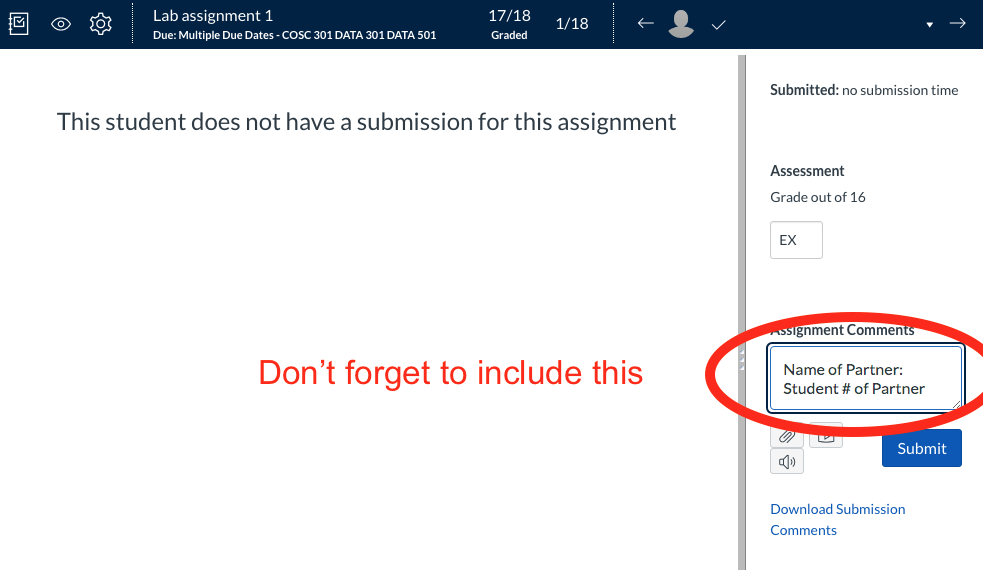
\includegraphics[width=0.9\textwidth]{img/partner.png}\\
\caption{Each partner should submit the name and student number of their partner in the assignment comments on Canvas.  {\bf Only one} partner should upload the files of the complete assignment.}
\label{default}
\end{center}
\end{figure}

\end{frame}






\begin{frame}{Evaluation}{}
DATA 301/COSC 301
\begin{center}
\begin{tabular}{|l|r|l}
\cline{1-2}
Clickers & 5\% & (in class) \\
Assignments & 30\% & (weekly-ish)\\
Two Midterms & 30\% & (in class) \\
Final Exam & 35\%  & (cumulative, 3 hours)\\
\cline{1-2}
\end{tabular}
\end{center}
\vfill
DATA 501 Graduate Student Evaluation:
\begin{center}
\begin{tabular}{|l|r|l}
\cline{1-2}
Project & 30\% & (Details to be posted on Canvas)\\
Two Midterms & 30\% & (in class)\\
Final Exam & 40\%  & (cumulative, 3 hours)\\
\cline{1-2}
\end{tabular}
\end{center}
\end{frame}

\begin{frame}
\frametitle{Midterms}
As stated on the TentativeSchedule (posted on \href{https://canvas.ubc.ca/}{Canvas}), midterms are held in class on:
\begin{description}
\item[Midterm 1] Tuesday, Feb 25, 2020
\item[Midterm 2] Thursday, March 26, 2020
\end{description}
\medskip

\begin{alertblock}{Clause}
A student must pass the final exam, or receive an average grade of at least 50\% on the exams (midterms and final) to pass the course. Otherwise, the student will be assigned a maximum overall grade of 45.  See table for examples:
\end{alertblock}
%\begin{itemize}
%\item Eg. midterm 1, 2, and final grade of 70\%, 35\%, and 45\%, resp., you would satisfy this clause.
%\item Eg. midterm 1, 2, and final grade of 70\%, 35\%, and 45\%, resp., you would satisfy this clause.
%\end{itemize}
\begin{center}
\begin{tabular}{|c|c|c|c|c|}
\hline
Midterm 1 & Midterm 2 & Final & Average Grade&Satisfy Clause \\
\hline
70\% & 35\% & 45\% & \textcolor{Green}{50\%} & \textcolor{Green}{Yes} \\
40\% & 35\% & \textcolor{Green}{50\%} & 42\% & \textcolor{Green}{Yes} \\
45\% & 51\% & 45\% & \textcolor{Red}{47\%} & \textcolor{Red}{No} \\
\hline
\end{tabular}
\end{center}

\end{frame}



%\begin{frame}{Evaluation}{}
%DATA 301/COSC 301
%\begin{center}
%\begin{tabular}{|l|r|l}
%\cline{1-2}
%Clickers & 5 \% & \\
%Assignments & 20 \% & (weekly-ish)\\
%Two Midterms & 30 \% & (in class) \\
%Final Exam & 45 \%  & (cumulative, 3 hours)\\
%\cline{1-2}
%\end{tabular}
%\end{center}
%\vfill
%DATA 501 Graduate Student Evaluation:
%\begin{center}
%\begin{tabular}{|l|r|l}
%\cline{1-2}
%Clickers & 5 \% & \\
%Assignments & 15 \% & (Bonus questions mandatory)\\
%Project & 10 \% & (Details to be posted on Canvas)\\
%Two Midterms & 30 \% & (in class)\\
%Final Exam & 40 \%  & (cumulative, 3 hours)\\
%\cline{1-2}
%\end{tabular}
%\end{center}
%\end{frame}
%
%\begin{frame}{Evaluation}
%\begin{itemize}
%\item A student must either receive:
%\begin{itemize}
%\item a passing grade of 50\% or above on the final exam
%\item  an average grade of at least 50\% on the exams (midterms and final) to pass the course. 
%\end{itemize}
%\textcolor{red}{Otherwise, they will receive a maximum overall grade of 45.}
%\medskip
%\item For example if you receive a 34\% on midterm 1, a 70\% on midterm 2 and a 40\% on the final, you average grade would be calculated as (34+70+40)/3 = 48\%.  Since this is below 50\% you would fail the course.
%\medskip
%%\item As another example, if you fail both midterms with a 45\%, an exam mark of 60\% would give you an average test grade of (45+45+60)/3 =50\%.  In this case, your grade would be calculated according to the table given on the previous slide. 
%\end{itemize}
%\end{frame}



\begin{frame}{Grad students Final Project}
\begin{itemize}
\item There is no clicker, lab or assignment component for students enrolled in Data 501 (although it is recommended that you work through these assignments for practice).
\medskip
\item Graduate students enrolled in DATA 501 will be expected to complete a Final Project 
\medskip
\item This includes a hand-in written proposal, final paper, and in-class presentation (final week of class)
\medskip
\item Pay attention on Canvas for postings on checkpoint deadlines, rubrics, etc.
\end{itemize}
\end{frame}


\begin{frame}{Academic Dishonesty}
Cheating in all its forms is strictly prohibited and will be taken very seriously by the instructor. \medskip
  \begin{block}{Assignments}
You are expect to  submit original work done by you and acknowledge all sources of information or ideas while attributing them to others as required.
 \end{block}
  \begin{block}{Exams}
All exams are closed book, so no course materials should be present.
  \end{block}

\end{frame}

\begin{frame}{Academic Misconduct}
Students are responsible for informing themselves of the guidelines of acceptable and unacceptable conduct for graded assignments established by their instructors for specific courses, and of the examples of academic misconduct set out \href{http://www.calendar.ubc.ca/okanagan/index.cfm?tree=3,54,111,959}{here}.   Some main concerns include:
\begin{itemize}
\item Plagiarism, which is intellectual theft, occurs when an individual submits or presents the oral or written work of another person as his or her own. 
\item Submitting the same, or substantially the same, essay, presentation, or assignment more than once (whether the earlier submission was at this or another institution) unless prior approval has been obtained from the instructor(s) to whom the assignment is to be submitted.
\end{itemize}
\end{frame}



\begin{frame}{Disciplinary Measures}
 Academic misconduct that is subject to \href{http://www.calendar.ubc.ca/okanagan/index.cfm?tree=3,54,111,960}{disciplinary measures} \\
 \medskip
 Academic misconduct often results in a one-year suspension from the University and a notation of academic discipline on the student's record. However, disciplinary measures which may be imposed, singly or in combination, for academic misconduct include, but are not limited to, the following:
\begin{itemize}
\item a failing grade or mark of zero on the assignment or in the course in which the academic misconduct occurred
\end{itemize}
\medskip
Note that all incidents of suspected academic misconduct must be reported to the Dean's Office.
\end{frame}




\begin{frame}{Academic Dishonesty}
\begin{alertblock}{Don't cheat!}
Do not cheat, copy, or mislead others about what is your work. 
\end{alertblock}
\begin{itemize}
%\item Incidences of plagiarism or cheating usually result in a failing grade or mark of zero on the assignment or in the course.
\item Violations of academic integrity (i.e., misconduct)  may result in a mark of zero on the assignment or exam and more serious consequences may apply if the matter is referred to the President's Advisory Committee on Student Discipline.
\medskip
\item Careful records are kept in order to monitor and prevent recurrences. {\bf If you have any questions about how academic integrity applies to this course, please consult with your professor. }
\end{itemize}
\end{frame}



\begin{frame}{How to Pass This Course}
The most important things to do to pass this course:\medskip
  \begin{alertblock}{Attend class and labs}<2->
  \vspace{-2mm}
    \begin{itemize}
%    \item Read notes before class as preparation and try the questions.
\item<3-> Follow along and annotate the lecture notes in class.
    \item<4-> Participate in class exercises and questions.
%  \end{alertblock}
%
%  \begin{alertblock}{Attend the labs and do all lab assignments}
%    \begin{itemize}
\item<5-> Labs are for marks and are practice to learn the material for the exams.
    \end{itemize}
  \end{alertblock}
\uncover<6->{To get an ``A" in this course do all the above plus:}
  \begin{alertblock}{Practice on your own. Practice makes perfect.}<7->
\uncover<8->{Do more questions than in the labs.  Try the techniques on your own data sets.}
  \end{alertblock}
\end{frame}


\begin{frame}{Disclaimer}
 There is a wide variety in previous experience.
\begin{itemize}
\item Some material you may already know.  Help others!!
\item Build up your computer experience in labs and outside of class.
\item Third-year standing means that you know how to ``figure things out.''
\medskip
\end{itemize}
 The course will be very straightforward: 
              Do the work and practice the techniques to do well.

\end{frame}


\begin{frame}{Systems and Tools}
All required software is available on the lab computers in SCI 234.\medskip
If you have your own personal laptop, it is advised that you download the required software prior to class so that you can follow along with examples in lecture.
\begin{itemize}
\item Our first unit uses Excel.  A student download of Microsoft office is available \href{https://it.ubc.ca/software-downloads}{here} \\[1em]\medskip
\end{itemize}

Canvas will be used for accessing lectures, submitting assignments, posting marks, discussions, and more,\dots \medskip

\begin{itemize}
%\item This is a new(ish) system to UBC \medskip
\item Support for students is available \href{https://canvas.ok.ubc.ca/2018/04/30/support-for-students/}{here}
\end{itemize}

\end{frame}




\begin{frame}{The In-Class Quizzes}
\begin{itemize}
\item To encourage attendance and effort, 5\% of your overall grade is allocated to answering in-class clicker questions.
\medskip
\item These questions are answered electronically using a clicker.
\medskip
\item The clicker can be purchased at the bookstore.
\medskip
\item Please refer to the {\bf ClickerOrientation} file uploaded to the {\bf Supplementary Material} Canvas on how to use them.
\medskip
\end{itemize}
\end{frame}

\begin{frame}{Clickers}
\begin{itemize}
\item The clicker is personalized to you with your student number.
\medskip
\item At different times during all the lectures, questions reviewing material will be asked.  Responses are given using clickers.
\medskip
\item You must answer 80\% of the questions correctly to get the full 5\%.
%There will be at least 75 questions throughout the semester. 
 %Each question is worth 1 mark, and you need at least 30 right answers to get the full 5\%.  
% \begin{itemize}
% \item  There will be more than 30 questions throughout the semester so do not worry if you %must miss a class or two or 
% forget your clicker one day!
% \end{itemize}
\medskip
\item There are some (not-for-grading) example clicker questions at the end of the lecture (I will take them up next class to ensure everyone has a chance to obtain a clicker first)
\end{itemize}
\end{frame}

\begin{frame}{Don't forget to register your clickers on Canvas}
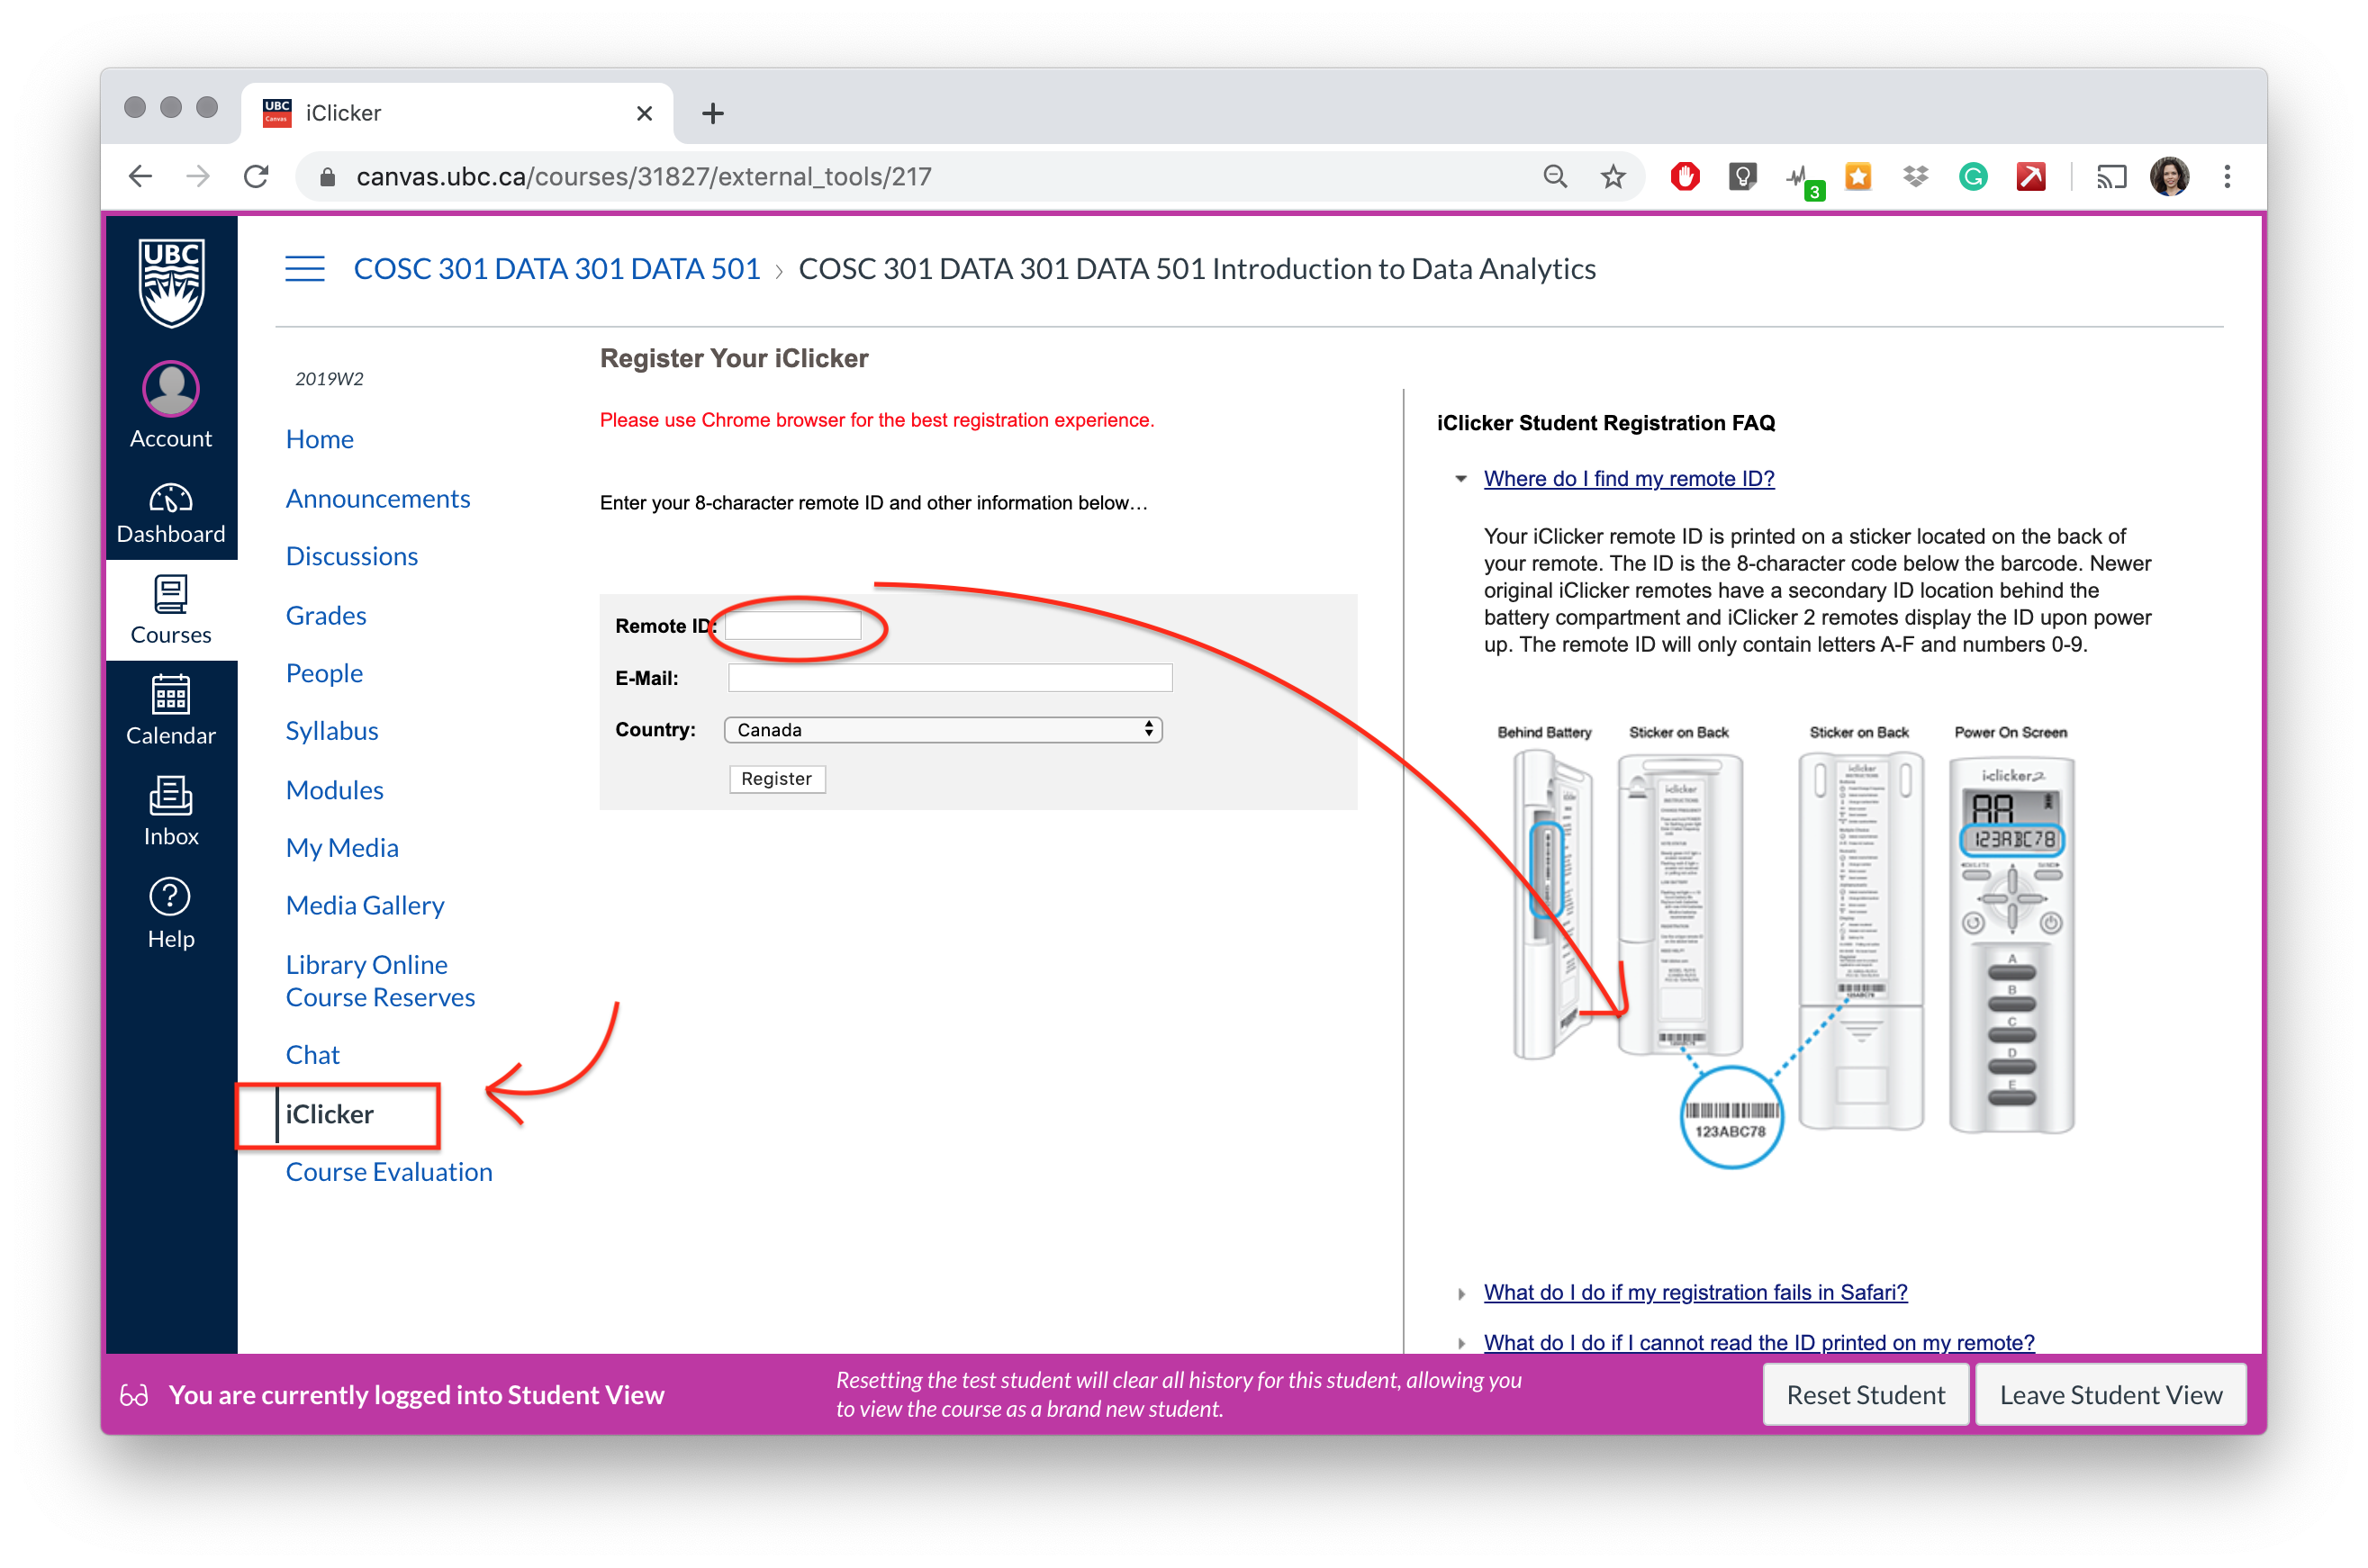
\includegraphics[width = 1.1\textwidth]{../SuppMat/clickerCanvas.png}
\end{frame}






\section
  {Intro to Data Analytics}

  \begin{frame}
\begin{center}
\textcolor{blue}{\Large An Introduction to Data Analytics}
\end{center}
  \end{frame}

  
  \begin{frame}{Data Analytics vs Data Analytics}
  \begin{block}{Data analysis}
  \emph{Data analysis} is the processing of data to yield useful insights or knowledge.
  \end{block}
  
  \begin{block}{Data Analytics}
    \emph{Data Analytics} is the science of examining raw data with the purpose of drawing conclusions about that information.\medskip
\end{block}


\end{frame}



% Differences Between Data Analytics vs Data Analysis
%Data analysis is a procedure of investigating, cleaning, transforming, and training of the data with the aim of finding some useful information, recommend conclusions and helps in decision-making. Data analysis tools are Open Refine, Tableau public, KNIME, Google Fusion Tables, Node XL and many more. Analytics is utilizing data, machine learning, statistical analysis and computer-based models to get better insight and make better decisions from the data. Analytics is defined as �a process of transforming data into actions through analysis and insight in the context of organisational decision making and problem-solving.� Analytics is supported by many tools such as Microsoft Excel, SAS, R, Python(libraries), tableau public, Apache Spark, and excel.

  \begin{frame}{Data Analytics vs Data Analytics}
  The distinction between data analysis and analytics is blurry to say the least (even \href{https://en.wikipedia.org/wiki/Analytics\#Analytics_vs._analysis}{Wikipedia} is confused).
  \vfill
  \href{https://www.getsmarter.com/blog/career-advice/difference-data-analytics-data-analysis/}{One source} might say that data analysis is a subcomponent of data analytics, while  \href{https://www.quora.com/What-is-the-difference-between-Analytics-and-analysis-data-analytics}{another source} says data analytics is a subcomponent of data analysis.
  \vfill
  I like to think of data analysis as the \textit{method} (ie \textit{action}) whereas data analytics are \textit{tools} used to do so.
  \vfill
  Analytics is supported by many tools such as Microsoft Excel,  SQL, Python, R, %Tableau
  all of which we will talk about in this course.
%  \begin{center}
%  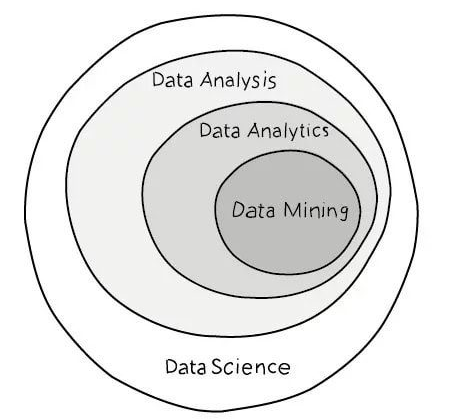
\includegraphics[width=0.5\textwidth]{dataanalytics.png}
%  Image source: \href{https://www.quora.com/What-is-the-difference-between-Analytics-and-analysis-data-analytics}{Quora}
%  \end{center}
\begin{center}

\includegraphics[height=1cm]{img/excel.png} \quad

\includegraphics[height=1cm]{img/sql}\quad

\includegraphics[height=1cm]{img/python}\quad

\includegraphics[height=1cm]{img/Rlogo}
%
\includegraphics[height=1cm]{img/Tableau}
\end{center}
  \end{frame}
  
    \begin{frame}{Other related terms}
% source: https://ca.simplilearn.com/data-science-vs-big-data-vs-data-analytics-article
Other terms that may add confusion to these definitions are \dots 
\begin{itemize}
 \setlength{\itemindent}{0em}
    \item \emph{Data Science} is a field comprised of everything  relating to data cleansing, preparation, and analysis. This umbrella term that encompasses data analytics, data mining, machine learning, and several other related disciplines. \medskip
    \item \emph{Big Data} usually refers to immense volumes of data  that inhibits the use of traditional data-processing applications. \medskip% and demands  cost-effective, innovative forms of information processing that enable enhanced insight, decision making, and process automation.
\end{itemize}
%\begin{tikzpicture}[remember picture,overlay]%[xshift=65mm,yshift=-48mm,anchor=north west]
%\node at (current page.center) {\includegraphics<handout:0>[width=.7\textwidth]{img/DataScientistTweet.png}};
%\end{tikzpicture}
\medskip
See \href{https://www.simplilearn.com/data-science-vs-big-data-vs-data-analytics-article}{this} article for more on the differences between Data Science, Big Data, and Data Analytics.
\end{frame}
% data analytics and big data are terms often used side-by-side, but they are not one in the same.
% If data science is the house that hold the tools and methods, data analytics is a specific room in that house. (https://insidebigdata.com/2017/06/03/difference-data-science-data-analytics/)


%  \begin{frame}{Massive Growth of Data - ``Big Data''}
%\emph{Big Data} is the general term used to describe the explosion of data collected and the opportunities to transform this data into useful insights to benefit society.\medskip
%\begin{itemize}
%\item "Big" enough to challenge how the data can be processed. \medskip
%\end{itemize}
%Some of the goals of big data analytics is to discover %of ?models? for
%meaningful patterns, extract information, draw conclusions and make decisions.
%\end{frame}


\begin{frame}{What is a Data Analyst?}
\begin{block}{Data analyst}
  A \emph{data analyst} is a person who uses tools and applications to transform raw data into a form that will be useful.
\end{block}
\begin{itemize}
\item Vital in a ``data-driven'' world with larger and more critical data sets.\medskip
%\medskip
%\item Data analyst jobs are projected to be one of the top jobs over the next 10 years, and this course has provided training in the skills needed for those jobs.
%\end{itemize}
%\end{frame}
%
%
%
%\begin{frame}
%  \begin{itemize}
  \item The first step in data analysis is often \emph{data collection/} \emph{munging/} \emph{processing} which involves finding, loading, cleaning, manipulating, transforming, %modeling,
   and visualizing the data.\medskip
\item The knowledge may be used for scientific discovery, business decision-making, or a variety of other applications.\medskip
  \end{itemize}
\end{frame}



  


\begin{frame}{Why is Data Analytics important?}
\emph{Data analytics} is important as society is collecting more and larger data sets all the time:\medskip
\begin{description}
\item[Web] All web pages visited and links clicked, searches made, images and posts\medskip
\item[Business] Items purchased by date, supply chain/customers, industrial sensors\medskip
\item [Science] Massive data sets (biological/genomic, astronomy, physics, healthcare)\medskip
\item [Environmental] Sensors and monitors (temperature, etc.) 
\end{description}
\end{frame}

\begin{frame}{Why is Data Analytics important?}
Transforming this raw data into useful insights has major value:\medskip
\begin{description}
\item [Web] Online advertising driven by understanding customer behaviour; \href{https://microarts.com/insights/why-googles-search-results-vary-from-person-to-person/}{tailored google searches}, \href{https://analytics.google.com/analytics/web/provision/?authuser=0\#/provision}{Google Analytics} \medskip
%When it comes to web analytics tools, Google Analytics is the gold standard. It�s simple to set up, customizable, and provides all the basic information you could want about your site. With Google Analytics, you can collect data on your audience (such as age, location, and devices), and observe how visitors find, interact with, and leave your site.  Source: https://searchenginewatch.com/2018/06/04/the-top-10-tools-for-getting-an-insight-into-your-website-analytics/
\item [Business] \href{https://channels.theinnovationenterprise.com/articles/how-sales-teams-are-using-predictive-analytics}{Sales predictions}, marketing promotions, manufacturing improvement\medskip
\item [Science] Scientific discoveries, new medical treatments and drugs; see some \href{https://www.datapine.com/blog/big-data-examples-in-healthcare/}{examples} in healthcare. \medskip
\item [Environmental] Understanding of environmental processes to allow for changing policies and behaviours, eg \href{https://www.the-iea.org/what-we-do/}{Institute of Environmental Analytics} \medskip
\end{description}
%See what Fitbit is doing with their data in \href{https://finance.yahoo.com/news/exclusive-fitbits-6-billion-nights-sleep-data-reveals-us-110058417.html}{this} article.
% eg, my fitbit tells me to get more sleep
% eg. prevent warming rivers by limiting tree cutting
\end{frame}




\begin{frame}{Why This Course is Important?}
\begin{itemize}
\item For many of you, this will be your first exposure to programming and data analytics.
\medskip
\item Regardless of your discipline, the tools you develop throughout this course will train you to think analytically and creatively.
\medskip
%https://www.quora.com/How-can-I-develop-critical-and-analytical-thinking-in-order-to-be-a-software-engineer
\item Beyond University, many professional jobs of the future will involve collecting, manipulating, and analyzing data. 
\medskip 
\item People who can understand how data can be used will have better employment opportunities. \medskip 
\end{itemize}
\end{frame}



\begin{frame}{Why This Course is Important?}
Important skills you may learn in this course:
\begin{itemize}
\item Excel Proficiency: %Everyone should know how to use Excel as a 
for general data analysis and productivity.\medskip
\item Databases: Understand how they work and how to use them.\medskip
\item Programming and Computational Thinking: Critical thinking and the ability to clearly articulate a problem in a systematic way has applications beyond data analytics.\medskip %become a more perceptive reader and listener, a more persuasive writer 
\item Applied Statistics: Using {\sf R} and other software makes your statistics training useful for real-world problems.\medskip
\item Data visualization: how to display and convey information in a meaningful way.
\medskip
\item Real-world problem solving: %Your toolkit will allow you to
learn to tackle real-world data analysis problems and understand %what tool to use and how to proceed.
when to use what tool.
\medskip
\end{itemize}
\end{frame}



 
 \begin{frame}{Data Analytics Toolkit}
 \begin{itemize}
 \item A data analyst has expertise in programming, statistics, data munging (transformation), and data visualization. \\
   \medskip % pronouced like mange (eat in intalian) -ing
 \item In this course, you will be introduced to severals tools for gaining competency in each of these skills. \\
\medskip
 \item As an introductory course, the goal is to get exposure to the skills and techniques as there will not be time for mastery.\\
 \medskip
 \item This toolkit of systems and techniques will be useful in many jobs even if they are not considered data analyst positions.
 \end{itemize}
 \end{frame}


  
  \begin{frame}{Why is Data Analytics important?}
\begin{itemize}
%\item Data analyst jobs are projected to be one of the top jobs over the next 10 years.
%See: {\tiny \url{http://blog.udacity.com/2014/11/data-analysts-what-youll-make.html}}
%\item In 2017, LinkedIn's Fastest-Growing Jobs Today Are In Data Science And Machine Learning {\tiny \url{https://www.forbes.com/sites/louiscolumbus/2017/12/11/linkedins-fastest-growing-jobs-today-are-in-data-science-machine-learning/#74f06bbc51bd}}
%\item More data will be created in 2017 than the previous 5,000 years of humanity \cite{AppDeveloper} \medskip
%
\item 90 percent of the worlds data have been generated over the last two years [\href{https://www.forbes.com/sites/louiscolumbus/2017/12/11/linkedins-fastest-growing-jobs-today-are-in-data-science-machine-learning/\#74f06bbc51bd}{Forbes Magazine}].
\medskip
\item In 2017, Machine Learning Engineers, Data Scientists, and Big Data Engineers ranked among the top emerging jobs on LinkedIn [\href{https://www.forbes.com/sites/louiscolumbus/2017/12/11/linkedins-fastest-growing-jobs-today-are-in-data-science-machine-learning/\#74f06bbc51bd}{Forbes Magazine}].
\medskip
\item  In 2012 was  Data Scientist dubbed the sexiest job of the 21st Century by \href{https://hbr.org/2012/10/data-scientist-the-sexiest-job-of-the-21st-century}{Harvard Business Review}.
\medskip
\item An estimated 2.7 million job postings for Data Analytics and Data Science are projected in the United States by 2020  [\href{https://www.ibm.com/downloads/cas/3RL3VXGA}{IBM}].
\end{itemize}
  \end{frame}
  
  



\begin{frame}{Massive Growth of Data - ``Big Data''}
Data facts from Forbes Magazine, May 21, 2018 [\href{https://www.forbes.com/sites/bernardmarr/2018/05/21/how-much-data-do-we-create-every-day-the-mind-blowing-stats-everyone-should-read/\#6c09172160ba}{Forbes}]
\begin{itemize}
%\item Over 90\% of the data in world history was created over the last two years.
\item An estimated 2.5 quintillion bytes (2.5 EB) generated per day.
%\item Global mobile data traffic estimated at 52 million TB and tripling by 2018.
\item Google processes about 3.5 billion requests/day and stores about 10 EB of data.
\item Facebook collects 500 TBs/day ($\sim$2.5 billion items) and stores 100+ PB of photos.
\end{itemize}
\medskip
 See \href{https://web-assets.domo.com/blog/wp-content/uploads/2017/07/17_domo_data-never-sleeps-5-01.png}{here} on how much data is generated every minute %(eg. 4,146,600 videos every minute on YouTube)
\begin{itemize}
\item Users watch 4,146,600 videos every minute on YouTube
\item Intagram users post 46,740 photos every minute.
\end{itemize}
\end{frame}




\begin{frame}{Types of Data Analysis}
\begin{description}
\item [Descriptive:] what are the features of the data? \medskip
\item  [Exploratory:] what new relationships/connections exist in the data?\medskip
\begin{itemize}
\vspace{-0.5em}
\item Correlation does not imply causation\medskip
% example murder rates and ice cream sales are highly positively correlated https://www.psychologyinaction.org/psychology-in-action-1/2011/10/30/what-is-a-confounding-variable
\end{itemize}
\item [Inferential:] use data samples to predict about larger population\medskip
\begin{itemize}
\vspace{-0.5em}
\item Statistical models: estimate value and uncertainty\medskip
\end{itemize}
\item [Predictive:] use data to predict values for other objects\medskip
\item [Causal:] what variables change values of other variables?\medskip
\begin{itemize}
\vspace{-0.5em}
\item Randomized studies: if give a drug/treatment, does it have a positive effect?
\end{itemize}
\end{description}
\end{frame}


% CLICKER slides
%\begin{frame}{Why are you here?}
%A) I want to learn more about data analytics.
%
%B) I know how important data is to my work or future work.
%
%C) I need an upper-year elective course.
%
%D) I already have training in computer science/statistics and want to expand my knowledge further.
%
%E) I want an easy credit.
%\end{frame}

%\begin{frame}{What topics are you most interested in?}
%A) Excel and SQL Databases
%
%B) Programming and Python
%
%C) Data Visualization and GIS
%
%D) R and Applied Statistics
%
%E) None of the above
%\end{frame}

%\begin{frame}{What is your major?}
%
%A) Math/Stat/Computer Science/Engineering
%
%B) Business
%
%C) Science (biology, chemistry, physics, environmental)
%
%D) Arts
%
%E) Other
%\end{frame}

%\begin{frame}{What is your Statistics background?}
%A) I have taken no statistics courses.
%
%B) I have taken a statistics course Ð not sure what I remember though.
%
%C) I have taken a statistics course and can explain what a confidence interval is.
%
%D) I have taken multiple statistics courses.
%\end{frame}

%\begin{frame}{What is your background with computers?}
%A) I can use computer and mobile applications
%
%B) I can write a formula in Excel
%
%C) I can write a simple program in some programming language
%
%D) I can write a query in SQL
%
%E) I am a CS major or have taken several CS courses
%\end{frame}




\begin{frame}{Clicker Test}
\begin{example}
Why are you here?
\begin{enumerate}[A)]
\item I want to learn more about data analytics.
\item  I know how important data is to my work or future work.
\item  I need an upper-year elective course.
\item  I already have training in computer science/statistics and want to expand my knowledge further.
\item I want an easy credit.
\end{enumerate}
\end{example}
\end{frame}

\begin{frame}{Clicker Test}
\begin{example}
Which of the following topics are you most interested in?
\begin{enumerate}[A)]
\item Excel and SQL Databases
\item Programming and Python
\item Data visualization and GIS
\item R and Applied Statistics
\item None of the above
\end{enumerate}
\end{example}
\end{frame}


\begin{frame}{Clicker Test}
\begin{example}
What is your major?
\begin{enumerate}[A)]
\item Math/Stat/Computer Science/Engineering
\item Buisness
\item Science (biology, chemistry, physics, environmental)
\item Arts
\item Other
\end{enumerate}
\end{example}
\end{frame}


\begin{frame}{Clicker Test}
\begin{example}
What is your computer background?
\begin{enumerate}[A)]
\item I can use computer and mobile applications
\item I can write a formula in Excel
\item I can write a simple program in some programming language (eg. Python, R, Java)
\item I can write a query in SQL
%\item I am a CS major or have taken several CS courses
\item Two or more of the above
\end{enumerate}
\end{example}
\end{frame}


\begin{frame}{Clicker Test}
\begin{example}
What grade are you expecting to get?
\begin{enumerate}[A)]
\item A
\item B
\item C
\item D
\item F
\end{enumerate}
\end{example}
\end{frame}



%\begin{frame}
%  {Pictures}
%
%  \begin{figure}[t]
%    \centering
%    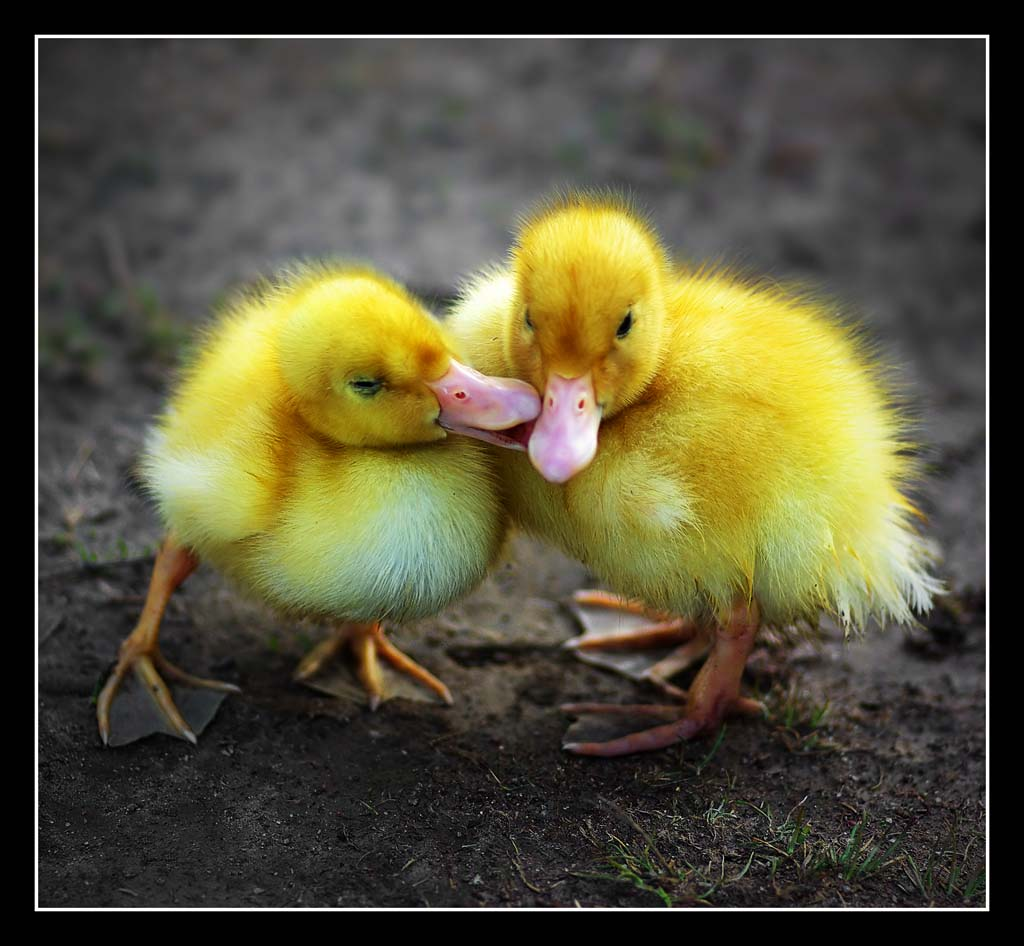
\includegraphics[height=\dimexpr11\textheight/16\relax]{ducks}
%    \caption{Kissing ducks}
%  \end{figure}
%\end{frame}


\end{document}

